
\chapter{Introducción}
\label{chap:introduction}
En este trabajo nos vamos a centrar en el problema de determinación de órbitas, que consiste en determinar los elementos orbitales de un cuerpo a partir de $N$ observaciones realizadas desde la Tierra y así poder situar dicho objeto en la bóveda celeste en cualquier momento. Concretamente, se estudiará el método de determinación Laplaciano, el cuál fue desarrollado en 1780 y que sirvió como base para los métodos que fueron apareciendo posteriormente.	Dado que vamos a trabajar con observaciones tomadas desde la Tierra, no conoceremos una parametrización del movimiento real del cuerpo cuya órbita determinar y por tanto nos serviremos del cálculo numérico con el fin de aproximar las cantidades que necesitemos para nuestro trabajo. Además, haremos un repaso de la mecánica celeste comentando los principales elementos que necesitaremos para nuestro estudio de determinación.\\

Una vez estudiado el método de Laplace, discutiremos el número de soluciones del problema que podemos obtener, buscando asegurar la unicidad y teniendo en cuenta que no todas las soluciones son válidas para nuestro problema físico. Por último, se desarrollará un programa que sea capaz de calcular la órbita de un cuerpo a partir de los datos introducidos de sus observaciones desde la Tierra, facilitando así la aplicación del método de Laplace.\\

El trabajo desarrollado en esta memoria está basado principalmente en el estudio de ``\textit{An Introduction to Celestial Mechanics}'', escrito por Forest Ray Moulton \cite{moulton}, así como en ``\textit{Introducción a la Mecánica Celeste}'' de Rafael Ortega Ríos y Antonio Jesús Ureña Alcázar \cite{ortega} y en los conocimientos adquiridos durante la carrera de cálculo numérico \cite{MNII}. Todas las imágenes utilizadas han sido construidas utilizando la herramienta online que proporciona el software matemático Geogebra \cite{geogebra} o generadas a través del programa implementado. Para el desarrollo informático se ha utilizado el lenguaje de programación Python, estudiado durante la carrera, junto a diferentes paquetes facilitados por el mismo lenguaje, y nos ha sido de gran ayuda la efemérides proporcionada por Jet Propulsion Laboratory (JPL) \cite{jpl}.\\

Pero, antes de entrar de lleno en las matemáticas, veamos un poco de historia sobre la determinación de órbitas.\\


\section{Una breve historia de la determinación de órbitas.}
\label{sec:history}
En 1687, Isaac Newton publica la primera edición de su obra \textit{Philosophiæ Naturalis Principia Mathematica}, más comúnmente llamado \textit{Principia}, dando el primer método de determinación de órbitas mediante tres observaciones, concretamente de órbitas parabólicas. Dicho método dependía de una construcción gráfica y una serie de aproximaciones sucesivas. Años más tarde, en 1705, Edmund Halley utilizó dicho método para calcular la órbita del cometa que lleva su mismo nombre, junto a otros cuerpos \cite{moulton}.\\

El primer método que apareció el cuál no dependía de una construcción gráfica fue dado en 1744 por Leonhard Euler. Aún así, hasta este momento los métodos estaban basados en mayor parte en suposiciones no del todo ciertas, por lo que Johann Heinrich Lambert intenta eliminar estas suposiciones y extiende el trabajo de Euler. Además, estudia la determinación para órbitas hiperbólicas y elípticas.\\

Durante años se siguen estudiando y desarrollando estos métodos, hasta que en 1780 Pierre-Simon Laplace publica un método completamente nuevo, el cual estudiamos en este trabajo, que se convierte en la base para muchos trabajos posteriores.\\

En el año 1801, Giuseppe Piazzi observa por primera vez el planeta enano Ceres durante un mes, obteniendo unas 20 observaciones de éste, aunque pronto se pierde su pista. Este hecho llama la atención al matemático Carl Friedrich Gauss, que comienza a desarrollar un método para encontrar los elementos orbitales de un objeto a partir de simples observaciones hechas desde la Tierra. Rápidamente Gauss resuelve el problema y un año más tarde H. W. Olbers y F. Von Zach, aplicando el método desarrollado, recuperan la órbita de Ceres ayudando a situar el cuerpo en la bóveda celeste de nuevo. Al igual que con el método de Laplace, este trabajo se convierte en un pilar para la determinación de órbitas. \cite{moulton}\\


Todos estos métodos son de hace siglos, por lo que la tecnología en ese entonces era muy limitada y las observaciones eran hechas con telescopios ópticos, tomando dos ángulos para situar el cuerpo observado pero sin poder conocer a priori la distancia del objeto. Actualmente, además de telescopios ópticos (mucho más avanzados que los que usaban Gauss o Laplace) se utilizan telescopios radar, y realizando las observaciones con estos dos tipos de telescopio en conjunto podemos conseguir la posición del objeto que observamos con mucha precisión, e incluso conocer la distancia y velocidad de éste gracias a los telescopios radar \cite{brett_r_wilson} \cite{vetter}. Esta mejora en las tecnologías de observación ha causado que se desarrollen nuevos problemas de determinación, en su mayor parte debido a la ingente cantidad de datos que se pueden obtener. \cite{gronchi}\\

La determinación de órbitas es un campo de estudio que tiene continuidad y actualmente sigue en uso, aunque con métodos mucho más modernos que el que desarrollaremos en este trabajo \cite{gronchi_unesco}. Uno de sus usos es para cartografiar el cinturón de asteroides, trabajo que (aparte de ser bonito) será muy importante en un futuro cuando comience la navegación espacial.\\


\section{Familiarizándonos con el problema.}
Como hemos comentado anteriormente, el método de Laplace fue desarrollado en el siglo XVIII, por lo que la instrumentación para la observación era limitada y surge una dificultad: observando un cuerpo desde la Tierra, la cuál se encuentra en continuo movimiento, podremos obtener la dirección del objeto percibida por el observador, sin ninguna información sobre su distancia. Al no disponer de esta distancia no podremos determinar su posición exacta, por lo que las componentes de la velocidad no podrán ser calculadas. Así, habremos de tomar observaciones complementarias. Pero, ¿cuántas necesitaremos, como poco, para obtener todos los elementos de la órbita?\\

A lo largo de esta memoria veremos que una órbita se define por seis elementos, por lo que nos bastará con que las observaciones nos proporcionen al menos seis valores independientes entre ellos. A partir de una observación completa obtenemos dos cantidades, referentes a las coordenadas angulares del cuerpo observado; por lo tanto, serán suficientes tres observaciones del objeto a determinar su órbita para comenzar nuestro proceso. Por otra parte, hay que tener en cuenta que, previo a nuestro estudio, podemos conocer algunos elementos de la órbita. Por ejemplo, si la órbita es parabólica\footnote{En este trabajo no se tratan las órbitas parabólicas de los objetos observados, y este ejemplo solo es ilustrativo de cómo podríamos utilizar menos de 3 observaciones completas a la hora de realizar la determinación de la órbita.}, conocemos su excentricidad ($e=1$), por lo que no serán necesarios seis elementos, sino cinco, y de esta manera una de las observaciones realizada puede ser dejada a medias, proporcionando solo una de las coordenadas angulares.\\

Las coordenadas angulares del cuerpo que observemos serán obtenidas en ascensión recta y declinación, un método de medida similar a la latitud y longitud utilizada sobre la superficie de la Tierra. Utilizaremos dichas coordenadas ya que la posición del cuerpo será determinada midiendo las distancias angulares y direcciones respecto a las estrellas vecinas, que se suponen fijas y están catalogadas en este tipo de coordenadas. Aún así, podremos cambiar a cualquier otro tipo de sistema de coordenadas cuando lo requiramos.\\

Comencemos viendo cuáles son los distintos elementos de una órbita, así como qué es la ascensión recta y declinación, que en conjunto llamaremos coordenadas ecuatoriales.\\





\section{Elementos Orbitales y Coordenadas Ecuatoriales}
\label{sec:orbital_elements_equatorial_coordinates}
En este apartado realizaremos un repaso a la mecánica celeste (objetivo 1), estudiando los diferentes parámetros que identifican una órbita (de manera única) así como las coordenadas ecuatoriales, elementos que forman un sistema que nos permite ubicar el objeto observado respecto al ecuador celeste y al equinoccio vernal (que definiremos más adelante) en un momento preciso.\\

\subsection{Elementos Orbitales}
\label{subsec:orbital_elements}
Comencemos por los elementos orbitales, los cuales necesitarán sostenerse en las dos primeras leyes de Kepler para ser desarrollados. Dichas leyes son:

\begin{enumerate}
\item \textit{Todos los planetas se desplazan alrededor del Sol describiendo órbitas elípticas, con el Sol en uno de los focos de dicha elipse.}
\item \textit{Cada objeto barre áreas iguales en tiempos iguales.}
\end{enumerate}

Pues bien, con esto comencemos a desarrollar nuestros elementos, entendiendo qué es una elipse y como se comporta matemáticamente.
\begin{definition}
La elipse es una curva plana, simple y cerrada, que consta de dos focos (puntos fijos) de manera que para cualquier punto de la curva que tomemos, la suma de las distancias de los focos a dicho punto es la misma. \cite{ortega}
\end{definition}

Llamando a nuestra elipse $E$ y a los focos de ésta $F_1$ y $F_2$, podemos escribir la definición superior de la siguiente manera:
\[
|x-F_1|+|x-F_2|=d, \; \forall x \in E \implies d>|F_1-F_2|
\]

Notar que en el caso de que $d=|F_1-F_2|$ estaremos ante un segmento que unirá los focos, mientras que si $0=|F_1-F_2|$, es decir, los dos focos son el mismo, nos encontraremos con que nuestra curva es una esfera.\\

Tomando uno de los focos como el origen de nuestro sistema de coordenadas, comencemos a desarrollar las ecuaciones anteriores. Sea $x$ un punto de la elipse, tenemos:
\[
|x|-|x-F|=d \implies |x-F|=d-|x| \implies |x-F|^2=(d-|x|)^2\\
\]

Como estamos trabajando con vectores, tenemos que $|x-y|^2=|x|^2+|y|^2-2\langle x,y\rangle$, denotando con $\langle\cdot,\cdot\rangle$ el producto escalar de dos vectores. Por tanto, continuando el resultado anterior:
\[
|F|^2-2\langle x,F\rangle=d^2+2d|x| \implies |x|-\frac{\langle x,F\rangle}{d}=\frac{d^2-|F|^2}{2d}
\]

Definimos así los valores $k\in\mathbb{R}$, que se corresponde con el factor de la derecha, $k=\frac{d^2-|F|^2}{d}$, y $\vec{e}\in\mathbb{R}^2$, $\vec{e}=-\frac{1}{d}F$. Por la desigualdad triangular, $|F|<|x|+|x-F|=d$, obtenemos que $|\vec{e}|<1$ y $k>0$. Por tanto, llegamos a la ecuación:
\begin{align}
|x|+\langle \vec{e},x\rangle=k,
\label{eq:elipse_cartesiana}
\end{align}

\noindent que será la ecuación que describe todas las elipses con un foco en el origen \cite{mecanica_celeste}.\\

\begin{figure}[H]
\centering
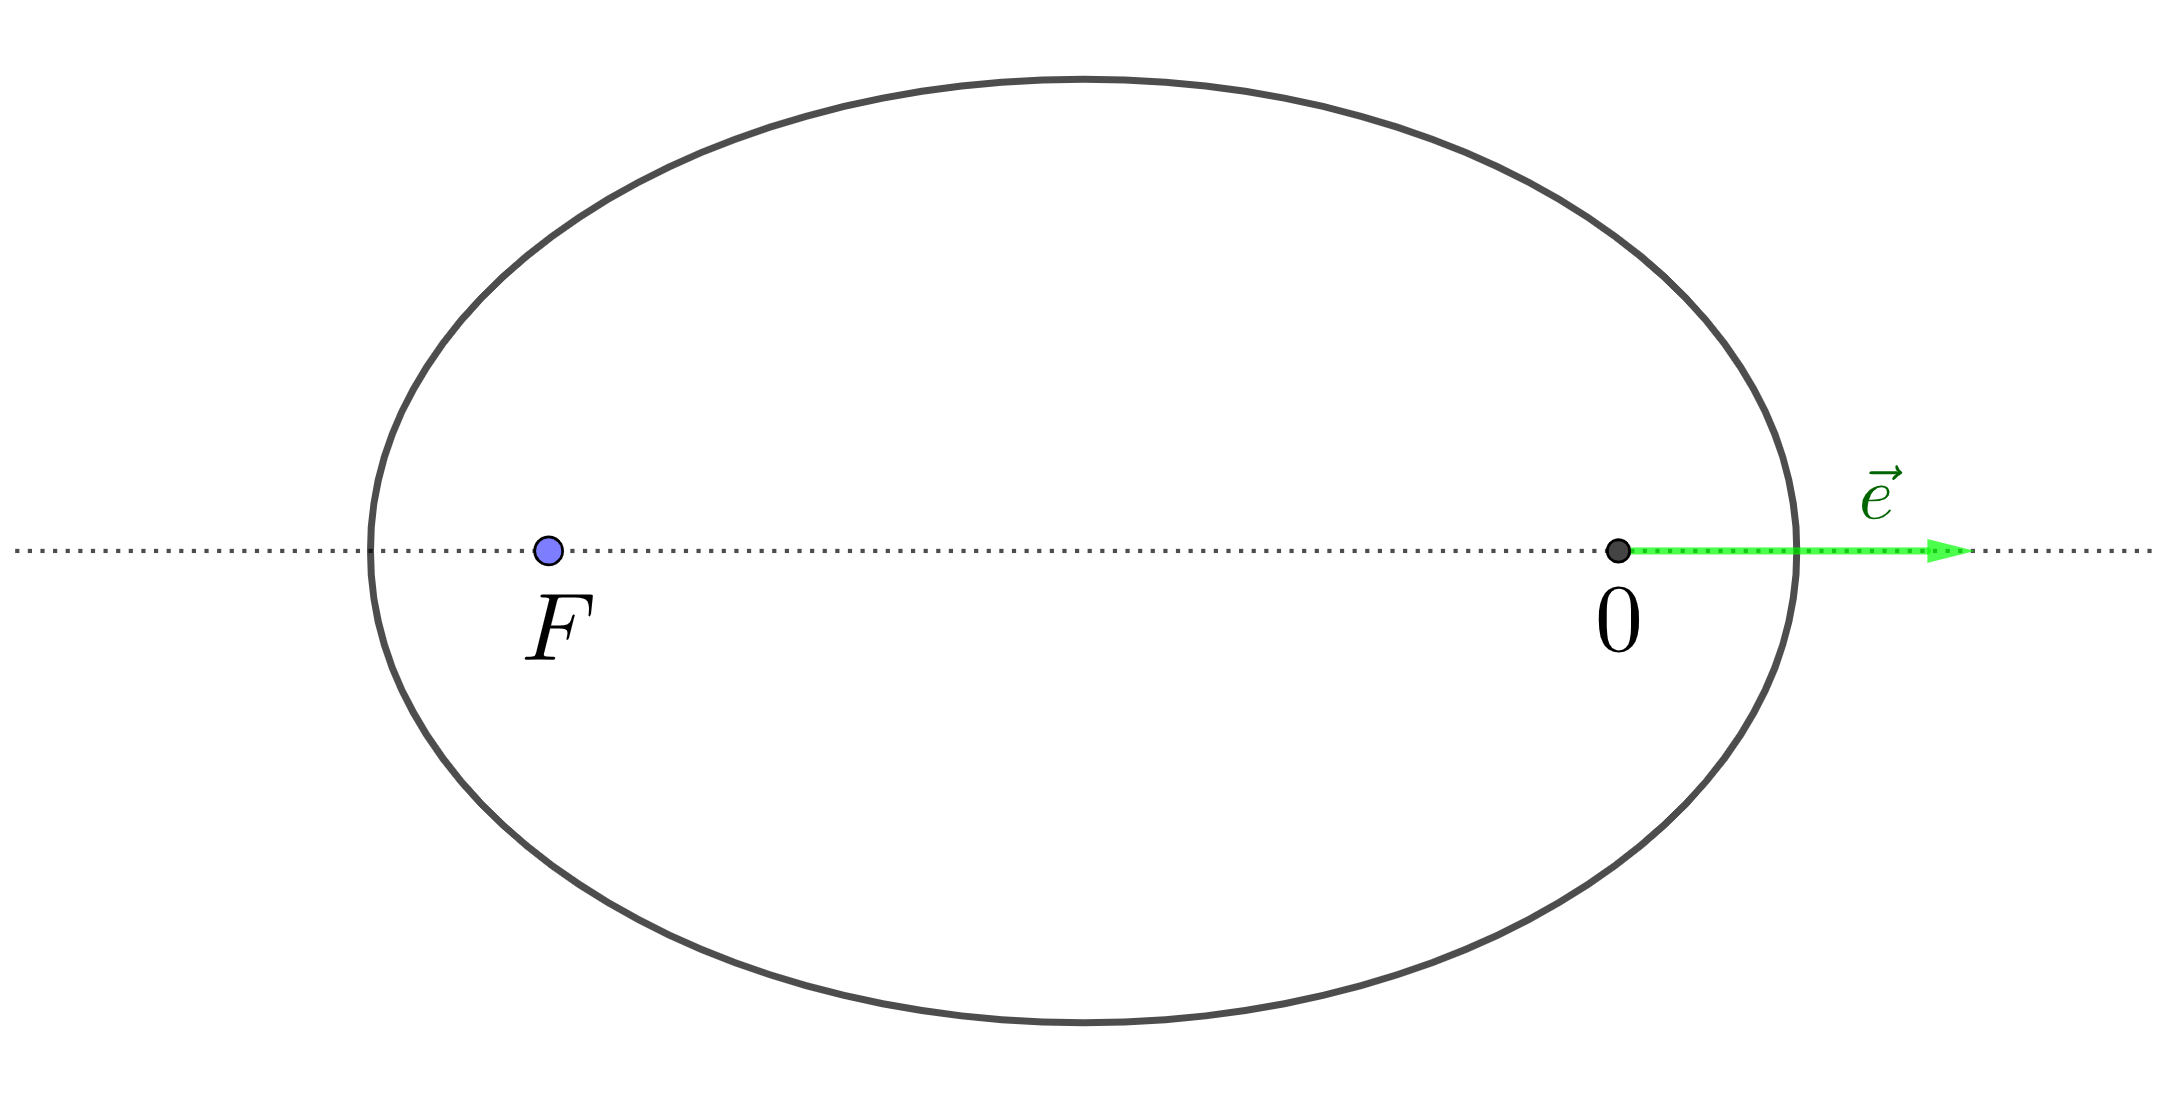
\includegraphics[scale=0.12]{images/elipse_excentricidad.png}
\caption{Representación de una elipse junto a sus focos y el vector $\vec{e}$.}
\label{fig:elipse_excentricidad}
\end{figure}

Llamaremos a $|\vec{e}|=e$ la \textbf{excentricidad de la elipse}, tomando valores en $[0,1[$. A mayor valor de excentricidad, mayor separación entre los focos, y viceversa. Si el valor de $e$ es 0, la curva que trazará el objeto será circular, los dos focos son iguales. Fuera del intervalo donde hemos definido la excentricidad, si $e=1$ la órbita del objeto es una parábola, y si es mayor que 1, el objeto describirá una órbita hiperbólica, aunque estos conceptos no serán necesarios para nuestro estudio de determinación.\\

Si trazamos una recta que pase por los dos focos de nuestra elipse, como podemos ver en \hyperref[fig:elipse_excentricidad]{la figura \ref{fig:elipse_excentricidad}}, dicha recta se intersecará con la elipse, obteniendo así dos puntos a los que llamaremos perihelio ($P$, más cercano a $0$) y afelio ($A$, más cercano a $F$). Si tomamos el centro de la elipse como el punto medio entre los dos focos y medimos la distancia desde el centro hasta el perihelio (o, equivalentemente, hasta el afelio), obtendremos el \textbf{semieje mayor} de la elipse, al que notaremos por $a$. Por otra parte, si trazamos una perpendicular a la recta que pasa por los focos que pase por el centro de la elipse, la distancia desde una de las intersecciones con la elipse hasta el centro nos dará el semieje menor, al que representaremos por $b$ \cite{ortega}. Podemos entender más fácilmente estos valores en la siguiente figura.

\begin{figure}[H]
\centering
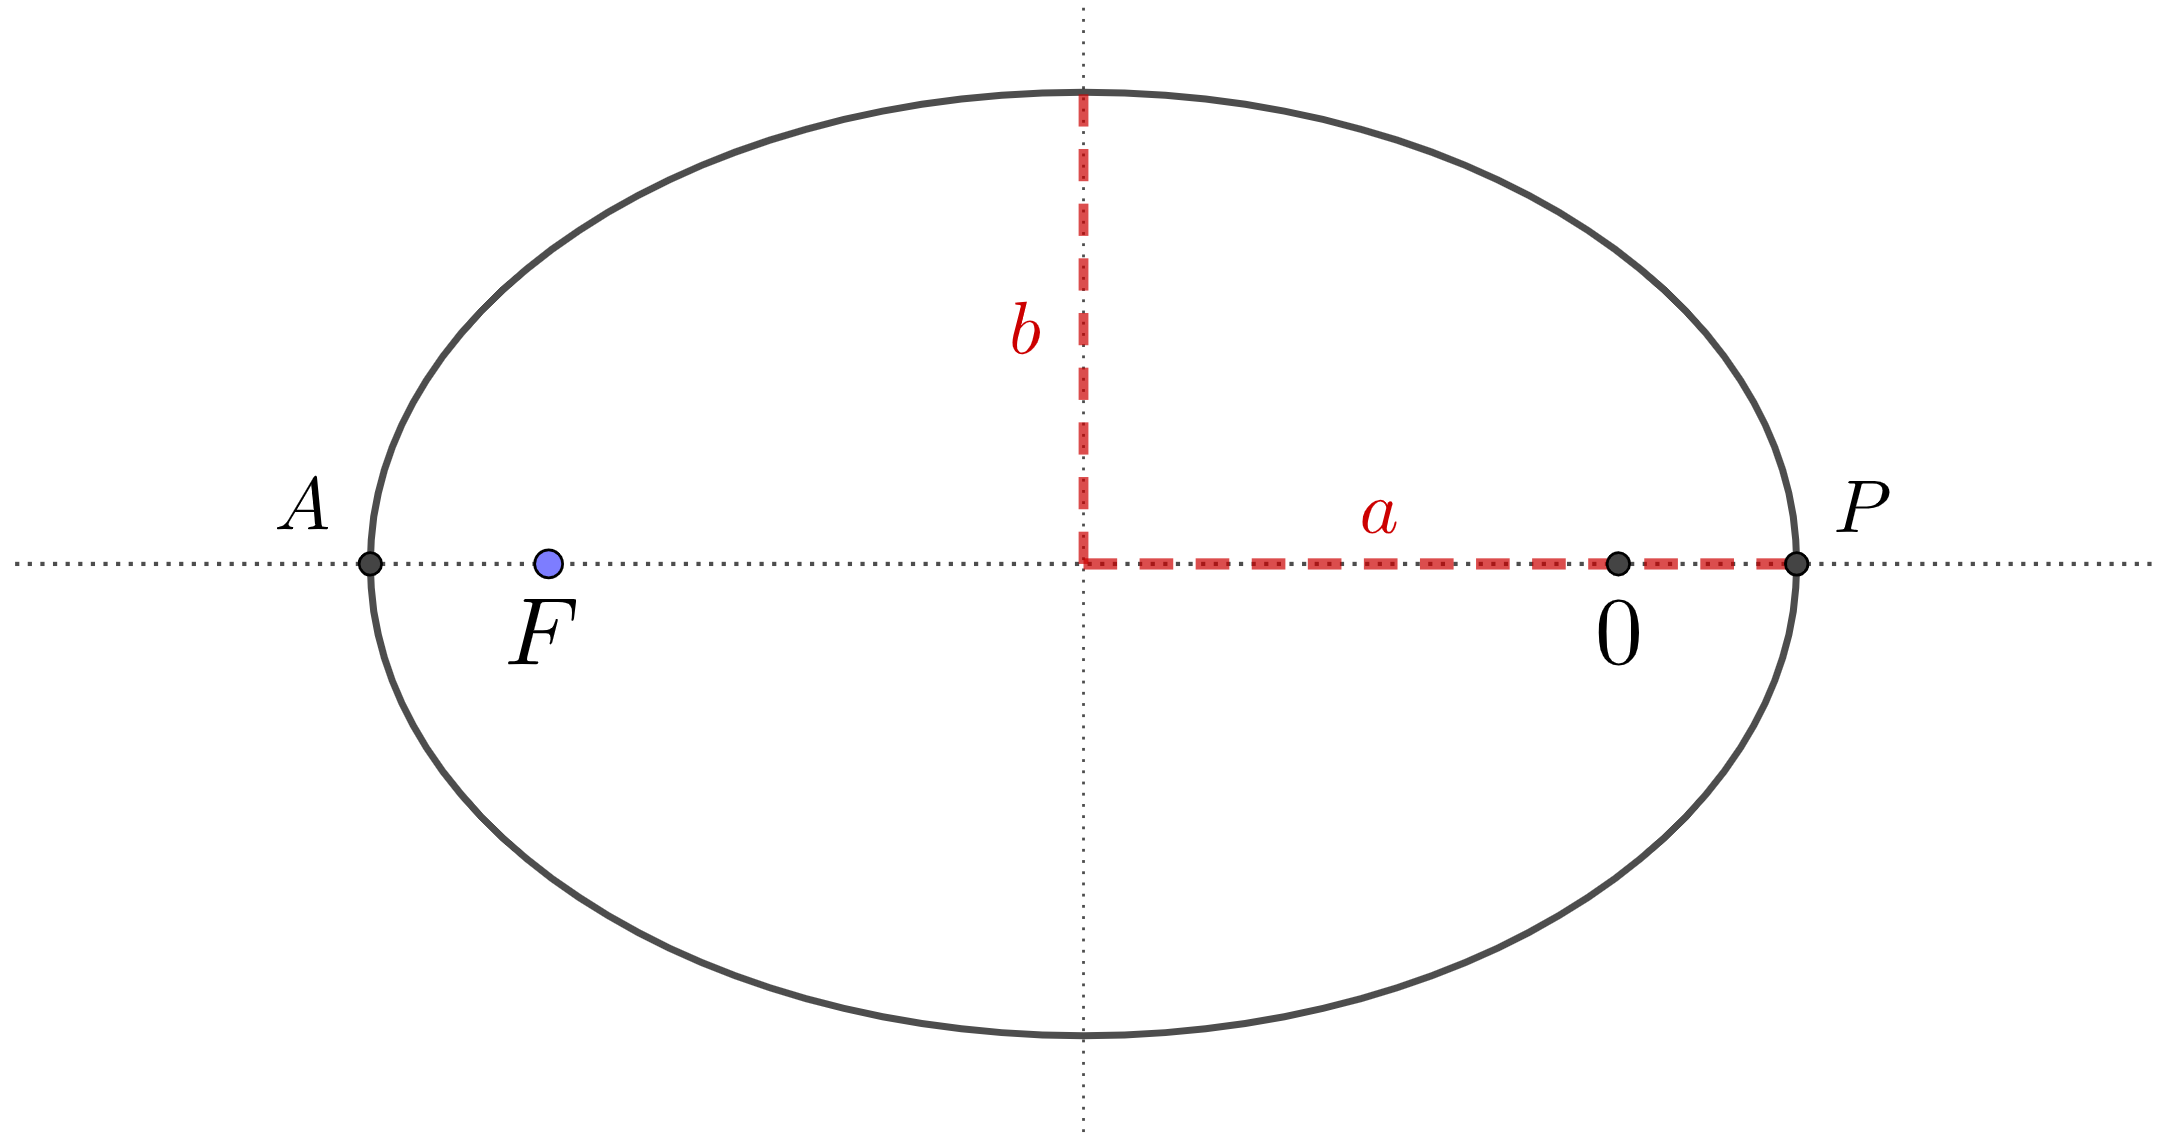
\includegraphics[scale=0.12]{images/perihelio_afelio.png}
\caption{Elementos geométricos de la elipse.}
\label{fig:perihelio_afelio}
\end{figure}


Notemos dos relaciones interesantes entre los elementos de la elipse comentados anteriormente y su excentridad:
\[
\frac{b}{a}=\sqrt{1-e^2}, \; \; \; \; \; \; \; \; \; \; \; \; \; \; \; \; \; \; \; \; e=\frac{\text{distancia entre los focos}}{\text{eje mayor}}=\frac{\overline{OF}}{2a}
\]

El punto donde se intersecan el semieje mayor y menor será el centro de la elipse, $C$, y podremos obtener una expresión de la distancia de cada uno de los focos a éste a partir de la segunda ecuación superior, sabiendo así que $\overline{0C}=\overline{FC}=ae$.\\

Por último, notemos por $\omega\in\mathbb{R}/2\pi\mathbb{Z}$ al \textbf{argumento del periastro}\footnote{El periastro toma diferentes nombres en función de qué objeto ocupe el foco 0, por ejemplo, si en dicho foco se encuentra el Sol lo llamaremos perihelio, si se encuentra la Tierra el perigeo, etc.}, que representará el ángulo formado entre el eje polar (equivalente al eje $x$ en el sistema cartesiano) y la dirección del vector $\vec{e}$. Así, tenemos que:
\[
\vec{e}=e(\cos{\omega},\sin{\omega})
\]

Llamemos $\mathcal{E}_0$ al espacio de elipses con foco en el origen, donde cada elipse queda determinada de manera única por su \hyperref[eq:elipse_cartesiana]{ecuación cartesiana}. Los parámetros $a$, $e$ y $\omega$ dan lugar a sistema de coordenadas en $\mathcal{E}_0$, que está definido sobre $\mathbb{R}^2$. Aquí surge un problema, pues las órbitas de los planetas son elipses en el espacio, cada una situada en un plano distinto, con un sentido de giro. Por tanto, será necesario definir un nuevo conjunto de parámetros para obtener un sistema de coordenadas sobre tres dimensiones.\\

Para empezar, definamos un sistema de referencia ortonormal en el espacio, que situará al Sol en el origen, y el plano $z=0$, en el que se encontrará el recorrido de la órbita de la Tierra, llamado plano de la eclíptica.\\

Empezamos definiendo el vector unitario $\vec{e}_3$, el cuál fijaremos como el normal al plano de la eclíptica. Dado que hay dos opciones (el normal positivo y el normal negativo), lo fijaremos a partir de la orientación que da el eje terráqueo de Sur a Norte. A continuación definimos $\vec{e}_1$, que tomamos en la recta formada por la intersección del plano del ecuador celeste con el plano de la eclíptica y dirección el punto vernal, situado en la constelación de Piscis\footnote{Antiguamente al punto vernal se le llamaba punto Aries debido a que la constelación a la que apuntaba era la constelación de Aries, pero durante los años dicho punto ha ido desplazándose hasta encontrarse apuntando a Piscis \cite{piscis}.}. Para terminar, escogemos el vector $\vec{e}_2$ como el vector ortonormal a $\vec{e}_1$ que está también en el plano de la eclíptica. Como de nuevo hay dos opciones, tomaremos el que de sentido positivo al giro de la Tierra (giro antihorario).\\

\begin{figure}[H]
\centering
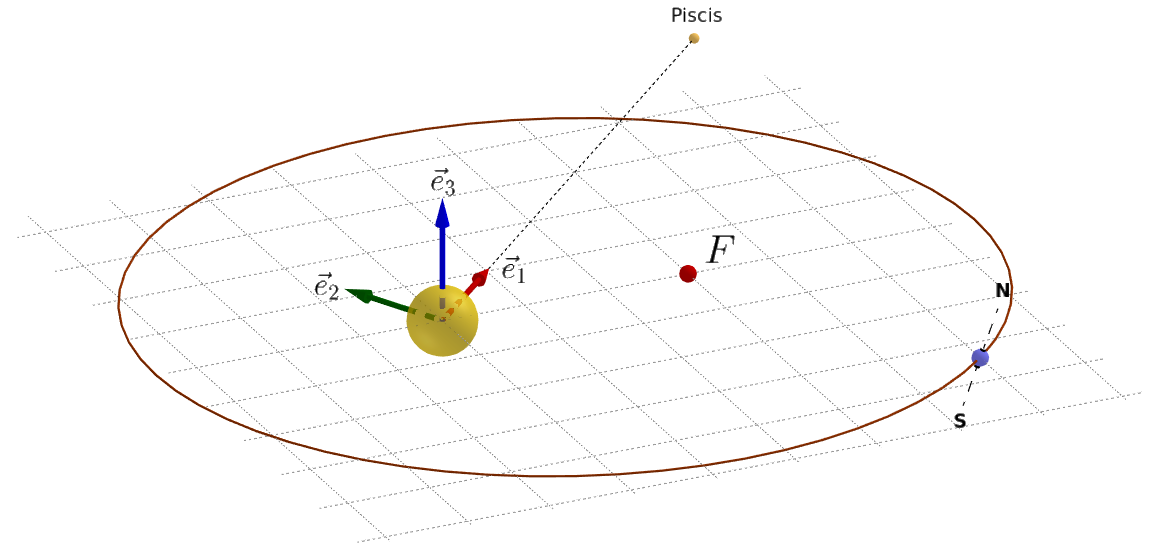
\includegraphics[scale=0.3]{images/sistema_coordenadas.png}
\caption{Órbita elíptica de la Tierra con focos $F$ y el Sol, mostrando el sistema de referencia. En la órbita terrestre real, el foco $F$ se encuentra dentro del Sol.}
\label{fig:sistema_referencia}
\end{figure}

Así, tenemos un sistema ortonormal $\{\vec{e}_1,\vec{e}_2,\vec{e}_3\}$ de manera que la orientación del movimiento de la Tierra se corresponde con la orientación $\{\vec{e}_1,\vec{e}_2\}$ del plano de la eclíptica \cite{mecanica_celeste}.\\

Para determinar una órbita elíptica por completo necesitaremos cinco elementos; $a$, $e$ y $\omega$ definidos anteriormente, y dos más que introduciremos a continuación que definirán el plano de movimiento: la \textbf{inclinación} respecto al plano de la eclíptica ($i$) y el \textbf{argumento del nodo ascendente} ($\Omega$).\\

Fijemos la línea de nodos como la recta que interseca el plano de movimiento del objeto observado y el plano de la eclíptica; sean $\vec{n}$ el vector normal al plano de movimiento, que es unitario y su sentido es el del momento angular, y $\mathcal{N}_+$ el lado positivo de la línea de nodos. Entonces:
\[
\left\{
\begin{array}{l}
	i=\measuredangle(\vec{e}_3,\vec{n}), \; \; \; \; \; \; \; \; \; \; i\in]0,\pi[\\
	\Omega=\measuredangle(\vec{e}_1, \mathcal{N}_+), \; \; \; \; \; \Omega\in\mathbb{R}/2\pi\mathbb{Z}
\end{array}
\right.
\]\\

Una vez hayamos definido el plano de movimiento con estos dos valores, encontramos la elipse usando la línea de nodos como eje de rotación para el argumento del perihelio, $\omega$.

\begin{figure}[H]
\centering
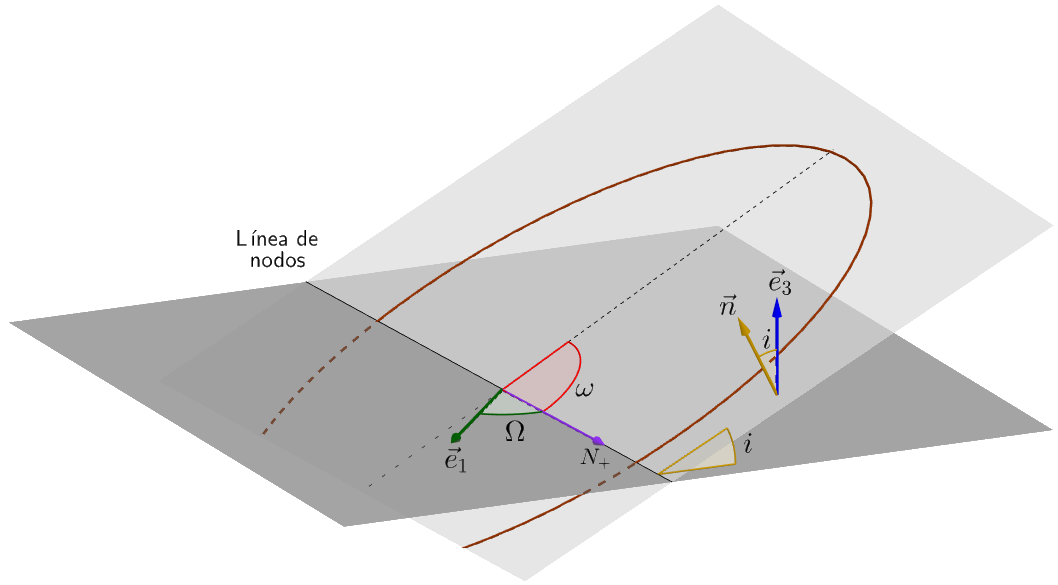
\includegraphics[scale=0.34]{images/omega_i.png}
\caption{Plano de movimiento del cuerpo definido por sus elementos orbitales.}
\label{fig:omega_i}
\end{figure}

Al conjunto de estas cinco coordenadas lo llamaremos \textbf{Coordenadas Astronómicas} o elementos orbitales, y están bien definidas y son unívocas en la región $i\in]0,\pi[$, $e\in]0,1[$, excluyendo así las órbitas circulares y las definidas sobre el plano de la eclíptica \cite{ortega}.\\

A estas cinco coordenadas podremos añadirle una sexta que por medio de la ecuación de Kepler nos permita determinar la posición del planeta para un momento $t$. Ese sexto elemento puede ser el valor $T$, que se define como el momento de paso por el perihelio, la fecha concreta del momento en el que el objeto está en el perihelio de su órbita. También puede ser usada la anomalía media, $M=n(t-T)$, con $n=\frac{2\pi}{p}$ el movimiento medio y $p$ el período de la órbita. Ésta representa la fracción del período de una órbita que transcurre desde que el cuerpo pasa por el perihelio hasta el momento $t$; obteniendo este ángulo podemos situar el objeto en el punto exacto de la órbita en el que se encuentra \cite{ortega}.\\

Cuando añadamos un sexto elemento a las coordenadas astronómicas tendremos que señalar una diferencia: si disponemos de cinco elementos, estaremos tratando la órbita como un lugar geométrico, mientras que añadiendo el paso por el perihelio (o la anomalía media) la estaremos tratando como una curva parametrizada donde se está describiendo el movimiento del cuerpo observado. Aún así, dado que para nuestro estudio lo que queremos es cartografiar las elipses, no necesitaremos el momento exacto del cuerpo en su órbita y utilizaremos solo cinco elementos. Veamos a continuación como, dadas estas coordenadas, podemos situar la elipse en el espacio.\\

\subsection{Situando la elipse que describe un cuerpo mediante sus coordenadas astronómicas.}
\label{subsec:set_ellipse_position}
Supongamos que se nos dan las coordenadas astronómicas $(a,e,i,\omega,\Omega)$ de un objeto y queremos situar su órbita en el espacio. Comenzaremos dibujando la elipse que forma su movimiento en el plano de la eclíptica, teniendo en cuenta que hemos de desplazar uno de sus focos para que éste se corresponda con el origen. Así, la ecuación para todos los puntos de la elipse en el plano se corresponderá con:
\[
(a\cos{\theta}+c, b\sin{\theta}, 0), \; \; \; \; \theta\in(0,2\pi)
\]

\noindent donde $a$ será el semieje mayor, $b=a\sqrt{1-e^2}$ el semieje menor y $c=ae$ la distancia de cada uno de los focos al centro de la elipse.\\

Por otra parte, $i$, $\Omega$, $\omega$ serán los ángulos de Euler \cite{euler_angles}, un conjunto de coordenadas angulares que utilizaremos para especificar la orientación del sistema de referencia del cuerpo con dichas coordenadas astronómicas en términos del sistema de referencia $\{e_1,e_2,e_3\}$ del plano de la eclíptica. Así, llamaremos $R$ al producto de las tres matrices de rotación siguientes:
\[
R=
\left(
\begin{array}{ccc}
	\cos{\omega} & \sin{\omega} & 0 \\
	-\sin{\omega} & \cos{\omega} & 0 \\
	0 & 0 & 1
\end{array}
\right)
\left(
\begin{array}{ccc}
	1 & 0 & 0 \\
	0 & \cos{i} & \sin{i} \\
	0 & -\sin{i} & \cos{i}
\end{array}
\right)
\left(
\begin{array}{ccc}
	\cos{\Omega} & \sin{\Omega} & 0 \\
	-\sin{\Omega} & \cos{\Omega} & 0 \\
	0 & 0 & 1
\end{array}
\right)
\]

\noindent y para situar la elipse en su plano de movimiento nos bastará multiplicar cada punto de ésta por la matriz $R$, obteniendo así que la órbita que sigue nuestro objeto en el espacio será:
\[
\text{Órbita}=R
\left(
\begin{array}{c}
a\cos{\theta}+c \\ b\sin{\theta} \\ 0
\end{array}
\right)
\]

Finalmente, si quisiéramos conocer el punto exacto de la elipse donde se encuentra el objeto en un momento $t$ habríamos de utilizar la anomalía media, $M$.\\


\subsection{Coordenadas Ecuatoriales}
\label{subsec:equatorial_coordinates}
Cada lugar en la Tierra puede ser localizado conociendo su latitud (ángulo en grados sobre el ecuador) y su longitud (ángulo en grados sobre el meridiano cero, el meridiano de Greenwich). De la misma manera, podemos definir ciertos valores para fijar la localización de todo objeto en la bóveda celeste, a los que llamaremos ascensión recta, $\alpha$, equivalente a la longitud, y declinación, $\delta$, equivalente a la latitud. A dichas coordenadas les acompañará un valor $\rho$ que determinará la distancia desde el observador hasta el objeto observado, aunque, como es de esperar, éste no puede ser obtenido con una simple observación del cuerpo.\\

Al igual que utilizamos una localización física en la Tierra como referencia para la longitud, utilizaremos el equinoccio vernal como referencia para la ascensión recta, que se encontrará en el punto de la eclíptica donde el Sol pasa del hemisferio sur al hemisferio norte, es decir, en la intersección del plano que pasa por el ecuador de la Tierra y del plano de la eclíptica. En dicho punto, la ascensión recta y declinación son nulas. A partir de la recta que une el centro de la Tierra con este punto se tomará el ángulo que forma con nuestro objeto observado. Para la declinación tomaremos el ecuador celeste, un gran círculo en la bóveda celeste en el mismo plano que pasa por el ecuador de la Tierra \cite{right_ascension_declination}.\\

\begin{figure}[H]
\centering
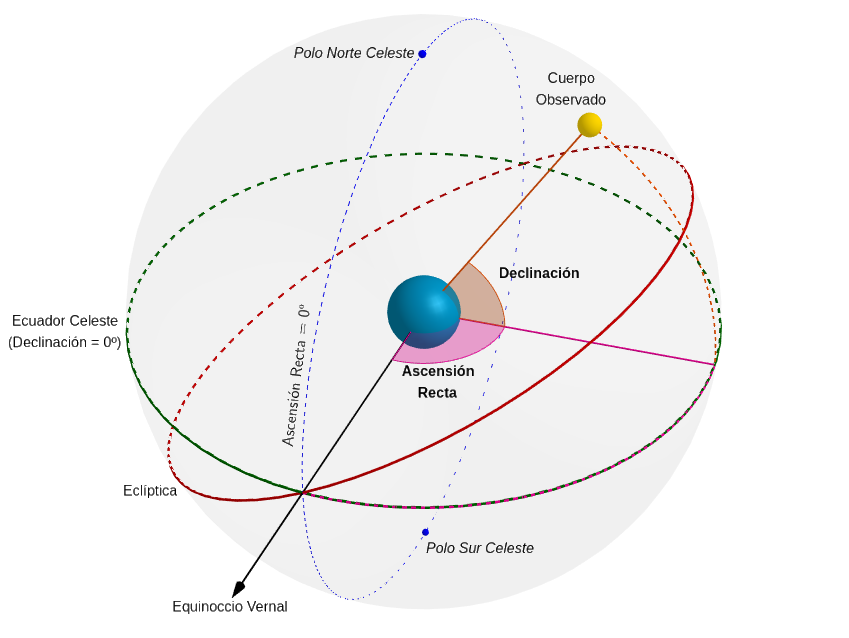
\includegraphics[scale=0.4]{images/ascension_declinacion.png}
\caption{La Tierra, en el centro, junto a la ascensión recta y declinación de cierto objeto. El círculo rojo define el camino aparente del Sol en el cielo, que define el plano de la eclíptica.}
\label{fig:ascension_declinacion}
\end{figure}

La declinación es medida en grados, como la latitud. Pero, a diferencia de la longitud, la ascensión recta es medida en horas, minutos y segundos en dirección este. Como en un día hay 24 horas, cada hora de ascensión recta corresponderá a una veinticuatroava parte de la rotación total de la Tierra, y por tanto, una hora será igual a $\frac{360}{24}=15º$.\\

Al conjunto de estas dos coordenadas junto a la distancia al objeto se les llama \textbf{Coordenadas Ecuatoriales}, y con ellas podremos definir la posición exacta de un objeto en cierto momento.\\

Dado que en ocasiones necesitaremos la posición del objeto en coordenadas cartesianas, veamos unas simples ecuaciones con las que pasaremos de coordenadas ecuatoriales a cartesianas \cite{moulton}.
\begin{align}
\left\{
\begin{array}{l}
	x = \rho \cos{\delta}\cos{\alpha}\\
	y = \rho \cos{\delta}\sin{\alpha}\\
	z = \rho \sin{\delta}
\end{array}
\right.
\label{eq:equatorial_to_cartesian}
\end{align}

Nótese que antes de aplicar estas ecuaciones deberemos pasar $\delta$ y $\alpha$ a radianes para utilizar las funciones trigonométricas. Las coordenadas $(x,y,z)$ tendrán la misma unidad que la distancia $\rho$.\\

\section{Caminos e ideas para desarrollar el método de determinación}
\label{sec:ideas_for_develope_method}
Una vez obtenidas las coordenadas ecuatoriales de un objeto mediante tres observaciones, las podemos escribir como un grupo de funciones de los elementos orbitales del cuerpo en el momento de las observaciones, $t_1, t_2, t_3$. Así, obtenemos lo siguiente:
\begin{align}
\left\{\begin{array}{l}
	\alpha_1 = \phi(a, e, \omega, i, \Omega, T; t_1)\\ 
	\alpha_2 = \phi(a, e, \omega, i, \Omega, T; t_2)\\ 
	\alpha_3 = \phi(a, e, \omega, i, \Omega, T; t_3)\\ 
	\delta_1 = \psi(a, e, \omega, i, \Omega, T; t_1)\\ 
	\delta_2 = \psi(a, e, \omega, i, \Omega, T; t_2)\\
	\delta_3 = \psi(a, e, \omega, i, \Omega, T; t_3)
\end{array}
\right.
\label{eq:ascension_declinacion}
\end{align}

Pues bien, el problema de determinación de órbitas consistirá en resolver todas estas ecuaciones para los seis elementos desconocidos, pero, las funciones de ascensión recta y declinación involucran a los elementos muy enrevesadamente, además de que son altamente trascendentales, es decir, no se pueden expresar en términos de funciones elementales.\\

La órbita a determinar podrá ser una elipse, una hipérbola o una parábola, y en los tres casos las coordenadas respecto a la Tierra se obtendrán mediante una serie de transformaciones trigonométricas, de manera que no dispondremos de soluciones directas para estas ecuaciones mediante métodos ordinarios.\\

El objetivo final del método de determinación es obtener la órbita del cuerpo observado, es decir, las coordenadas astronómicas que definen su movimiento. Pero, antes de todo, habremos de tratar el problema de encontrar cantidades intermedias con las que definir estas coordenadas, y como veremos más adelante (en \ref{subsec:orbital_elements}), a partir de la posición y la velocidad de un objeto en un instante $t$ se podrán obtener todos los elementos orbitales de éste.\\

Volvamos a las ecuaciones \eqref{eq:ascension_declinacion}, y supongamos que queremos encontrar las coordenadas polares y sus derivadas, por ejemplo, en $t=t_2$. Podemos reescribir las ecuaciones como:
\begin{align}
\left\{\begin{array}{l}
	\alpha_1 = f(\alpha_2, \delta_2, \rho_2, \alpha_2', \delta_2', \rho_2'; t_1, t_2)\\ 
	\alpha_2 = \alpha_2\\
	\alpha_3 = f(\alpha_2, \delta_2, \rho_2, \alpha_2', \delta_2', \rho_2'; t_2, t_3)\\
	\delta_1 = g(\alpha_2, \delta_2, \rho_2, \alpha_2', \delta_2', \rho_2'; t_1, t_2)\\
	\delta_2 = \delta_2\\
	\delta_3 = g(\alpha_2, \delta_2, \rho_2, \alpha_2', \delta_2', \rho_2'; t_2, t_3)
\end{array}
\right.
\label{eq:idea_laplace}
\end{align}

\noindent donde $\rho$ es la distancia al planeta en $t_2$ y:
\[
\alpha_2'=\frac{d\alpha}{dt}, \; \; \; \delta_2'=\frac{d\delta}{dt}, \; \; \; \rho_2'=\frac{d\rho}{dt} \; \; \;  \text{en} \; \; t=t_2
\]

Así, solo tendremos que resolver cuatro ecuaciones para cuatro incógnitas, pues $\alpha_2$ y $\delta_2$ son conocidas. Podremos modificar estas ecuaciones para hacer que sean más manejables a la hora de determinarlas, y, de hecho, este es el camino que toma \textbf{Laplace} a la hora de desarrollar su método, que fue aplicado por primera vez en 1780.\\

Por otra parte, podemos tomar tres coordenadas en dos momentos diferentes, $t_1$ y $t_3$, para así obtener otro conjunto de elementos a determinar, y haciéndonos así con dos ecuaciones con solamente dos incógnitas, que podrán ser resueltas.
\begin{align}
\left\{\begin{array}{l}
	\alpha_1 = \alpha_1\\
	\alpha_2 = F(\alpha_1, \delta_1, \rho_1, \alpha_3, \delta_3, \rho_3; t_1, t_2, t_3\\
	\alpha_3 = \alpha_3\\
	\delta_1 = \delta_1\\
	\delta_2 = G(\alpha_1, \delta_1, \rho_1, \alpha_3, \delta_3, \rho_3; t_1, t_2, t_3)\\
	\delta_3 = \delta_3
\end{array}
\right.
\label{eq:camino_gauss}
\end{align}

Este es el camino que siguió Lagrange para resolver el problema en 1778, y que retomó \textbf{Gauss} en 1801.\\

A pesar de la cantidad de estudios que se han realizado tras la publicación de estos métodos, muy poco de lo que es realmente nuevo o teóricamente importante se ha añadido a las determinaciones que desarrollaron Laplace y Gauss, a menos que se usen más de tres observaciones. \cite{moulton}\\


\section{Preparación y corrección de las observaciones}
Independientemente del método que queramos seguir para determinar la órbita del objeto observado, habremos de efectuar algunas correcciones en los datos obtenidos antes de comenzar a realizar cálculos, pues hay distintos factores que pueden hacer que la ascensión recta y declinación observadas difieran de su valor real.\\

En el equinoccio de primavera, que se corresponde con el punto Aries como comentamos anteriormente, la ascensión recta y declinación es nula, pues el plano de la eclíptica y el del ecuador de la Tierra se intersecan en dicho momento. Debido a la protuberancia de la Tierra en el ecuador, la Luna y el Sol causarán una ligera oscilación periódica y un lento cambio secular en la posición del plano de su ecuador. Así, los equinoccios no se corresponderán con un punto fijo y habrá pequeñas oscilaciones periódicas y lentos cambios de la posición de la Tierra a lo largo de la eclíptica, llamadas nutación y precesión. En este caso, se acostumbra a utilizar el equinoccio medio (equinoccio prescindiendo de la nutación) y la posición del ecuador al comienzo del año en el que se estén haciendo las observaciones para evitar el error en la ascensión recta y declinación.\\

Por otra parte, la observación del objeto cuya órbita queremos determinar también puede ser afectada por la aberración de la luz, es decir, la diferencia entre la posición observada del objeto y su posición real, causada por la combinación de la velocidad del observador (por la rotación de la Tierra) y la velocidad de la luz. Tendremos que corregir dos aberraciones: la anual, debida a la rotación de la Tierra alrededor del Sol, y la aberración diurna, debida a la rotación de la Tierra sobre su eje. Aún así, debido a que la velocidad de rotación sobre su eje es muy pequeña en comparación con la velocidad de traslación, la aberración diurna será relativamente pequeña, y podrá ser obviada, especialmente en el caso de que las observaciones tomadas no sea demasiado precisas. \cite{moulton}\\

Aunque no veamos la manera de hacer las correcciones sobre nuestras observaciones en este trabajo, es un paso a la hora de determinación muy importante y que deberá de ser gestionado en el momento que se quiera hacer una determinación de la órbita de un objeto mediante observaciones por telescopio.\\


\iffalse
\begin{comment}
Definamos como $\alpha_0$ y $\delta_0$ la ascensión recta y declinación del cuerpo observado en cierto momento, sin ninguna corrección previa. Entonces, sus valores referidos al equinoccio medio del comienzo del año, y corregidos para la aberración lumínica anual, son:
\[
\left\{
\begin{array}{l}
	\alpha = \alpha_0 - 15f - g \sin(G+\alpha_0) \tan(\delta_0) - h \sin(H+\alpha_0) \sec(\delta_0)\\
	\delta = \delta_0 - i \cos(\delta_0) - g \cos(G+\alpha_0) - h \cos(H+\alpha_0) \sin(\delta_0)
\end{array}
\right.
\]

\noindent donde $f, g, h, G$ y $H$ son cantidades auxiliares, a las que llamaremos \textit{números interestelares independientes}, y cuyo valor aparece en el \textit{American Ephemeris and Nautical Almanac} para cada día del año. Notar que estas correcciones serán expresadas en segundos de arco, pues en esta unidad son dadas las cantidades tomadas de la efemérides. Esta corrección será pequeña siempre que $\delta_0$ no sea cercano a $\pm90º$, pues cerca de dichos valores tanto la secante como la tangente que aparece en la corrección para $\alpha$ diverge.\\

Por último, tendremos que corregir la aberración diurna a través de las siguientes ecuaciones:
\[
\left\{
\begin{array}{l}
	\Delta \alpha = -0''.322 \cos(\phi) \cos(\theta - \alpha_0) \sec(\delta_0)\\
	\Delta \delta = -0''.322 \cos(\phi) \sin(\theta - \alpha_0) \sin(\delta_0)
\end{array}
\right.
\]

\noindent donde $\phi$ representará la latitud del observador y $\theta-\alpha_0$ representa el ángulo horario del objeto en el momento de la observación (\textit{???}). La primera corrección será pequeña mientras que $\delta_0$ no sea cercano a $\pm90º$, y la segunda no podrá exceder el valor de $0''.322$.\\

\textit{DUDAS: como se utilizan las dos correciones a la vez???? $0''.322$ se refiere a 0.322 segundos??}\\
\end{comment}
\fi


\section{Argumentación general para la determinación}
Los dos métodos más importantes para la determinación (Laplace y Gauss) siguen una estrategia similar, que expondremos a continuación. Para empezar, supongamos que solo disponemos de tres observaciones de nuestro objeto en tres momentos diferentes, $t_1, t_2, t_3$, de manera que conocemos la ascensión recta y declinación en cada uno de estos instantes. A continuación, definamos algunos términos:
\begin{itemize}
\item Definimos $C$, $S$ y $E$ como el cuerpo observado, el Sol (alrededor del cual gira $C$) y la Tierra respectivamente.
\item Sean $(\xi,\eta,\zeta)$ las coordenadas (cartesianas) de $C$ respecto a $E$, $(X,Y,Z)$ las coordenadas de $S$ respecto a $E$, y $(x,y,z)$ coordenadas de $C$ respecto a $S$.
\item $\rho$ es la distancia de $E$ a $C$, $r$ la distancia de $S$ a $C$ y $R$ la distancia de $E$ a $S$.
\end{itemize}

\begin{figure}[H]
\centering
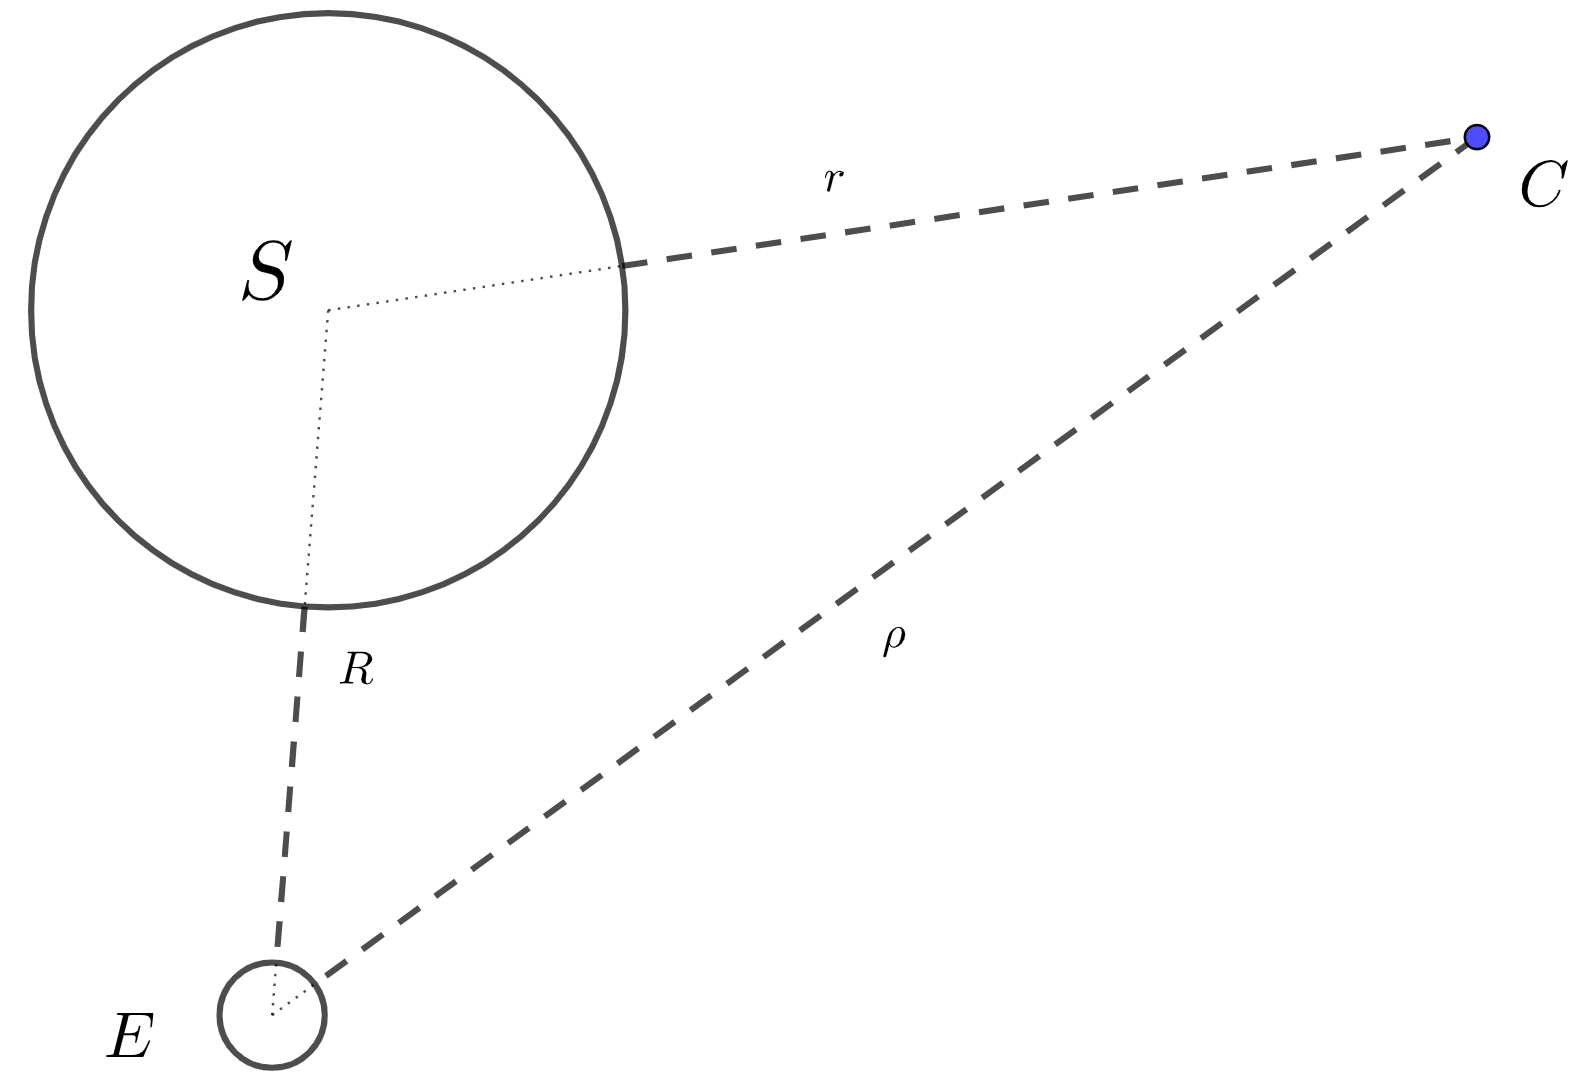
\includegraphics[scale=0.15]{images/notation.png}
\caption{Notación utilizada para nuestro problema}
\label{fig:notation}
\end{figure}

Con todo esto, podemos escribir:
\begin{align}
\left\{
\begin{array}{l}
\xi = \rho \cos{\delta}\cos{\alpha} = \rho\lambda\\
\eta = \rho \cos{\delta}\sin{\alpha} = \rho\mu\\
\zeta = \rho \sin{\delta} = \rho\nu
\end{array}
\right.
\label{eq:terminologia}
\end{align}
\noindent donde $(\lambda,\mu,\nu)$ es un vector unitario conocido que apunta de la Tierra al cuerpo observado, y el fin del estudio del problema será determinar $\rho$. \cite{moulton}\\

\section{Cambios en el plano de referencia.}
\label{sec:reference_plane}
Actualmente, la IAU (\textit{International Astronomical Union}) utiliza como sistema de coordenadas estándar el sistema ICRS (\textit{International Celestial Reference System}), del cuál deriva el plano ICRF (\textit{International Celestial Reference Frame}). De esta manera, a la hora de tomar la ascensión recta y declinación de un cuerpo lo obtendremos en el plano de referencia de la efemérides, es decir, en ICRF. El problema surge de que nuestro sistema de coordenadas tiene como base el plano de la eclíptica, que difiere de plano ICRF, y por tanto, tras obtener la posición y velocidad del cuerpo observado habremos de modificar las coordenadas para disponer de ellas en función del plano de la eclíptica \cite{ICRF}.\\

Para ser coherente con el ICRS y el origen de este (el baricentro del Sistema Solar), definimos el plano de la eclíptica como un plano que pasa por el origen del ICRS con una inclinación $\varepsilon_0$, que se corresponderá con la oblicuidad media, la inclinación del eje de la Tierra respecto al plano de la eclíptica \cite{ICRF} ($\approx23.4375º$ \cite{jpl}). Así, la transformación de las coordenadas del plano ICRF $(x,y,z)$ al plano de la eclíptica $(X,Y,Z)$ será:
\begin{align}
\left\{
\begin{array}{l}
	X=x\\
	Y=y\cos{\varepsilon_0}+z\sin{\varepsilon_0}\\
	Z=-y\sin{\varepsilon_0}+z\cos{\varepsilon_0}\\
\end{array}
\right.
\label{eq:ICRS_to_ecliptic}
\end{align}




\newpage
\thispagestyle{empty}


